\documentclass[11pt]{article}

\usepackage{graphicx}
\usepackage{epstopdf}
\hoffset        2mm 
\voffset        -15mm
\oddsidemargin  0mm
\topmargin      0.5in
\textwidth      6in
\textheight     9in

\begin{document}

\begin{titlepage}

\vspace*{55mm}
\begin{center}
{\huge MATH609-600}\\[1cm]
{\em \huge Programming Assignment \#2}\\[70mm]
{\large Fall, 2015} \\[15mm]
\end{center}

\begin{flushright}
{\LARGE Hasan Tahir Abbas}
\end{flushright}

\vfill

\end{titlepage}

\newpage
\section{Problem Specifications}
The compututional examples are explored using basic iterative methods.


\subsection{System with a Tridiagonal matrix}

The approximate solution of the given linear system is computed for various intervals and iterative methods and then compared with the exact solution in the first part.

\begin{table}[!hbt]
\begin{center}
{\def\arraystretch{.95}
\begin{tabular}{|c|c|c|c|}
\hline
Method & $n = 19$  &  $n = 39$  &  $n = 79$\\
\hline
Jacobi & 1915 & 7222& 27078\\ 
\hline
Gauss-Seidel & 977 & 3679 & 13788\\
\hline
SOR & 426 & 1632 & 6150\\
\hline
SSOR & 240 & 839 & 3144\\
\hline
\end{tabular}}
\end{center}
\caption{Iterations for Convergence required in Example 1, part a}
\end{table}
%%%%%%%%%%%%
\begin{table}[!hbt]
\begin{center}
{\def\arraystretch{.95}
\begin{tabular}{|c|c|c|c|}
\hline
Method & $n = 19$  &  $n = 39$  &  $n = 79$\\
\hline
Jacobi & 1914 & 7225& 27115\\ 
\hline
Gauss-Seidel & 976 & 3679 & 13803\\
\hline
SOR & 425 & 1631 & 6153\\
\hline
SSOR &358 & 1064 & 3546\\
\hline
\end{tabular}}
\end{center}
\caption{Iterations for Convergence required in Example 1, part b}
\end{table}


\subsection{Approximation of 2D Elliptic equation}

A 5-point finite difference formula is used to model the two-dimensional elliptic equation. The approximate solution is computed by applying the given boundary conditions.\\
In general, SSOR converges at the fastest rate to the required tolerance level. However, due to certain requirements on the matrix to be inverted, it does not alwasys give the correct results.

\begin{table}[!hbt]
\begin{center}
{\def\arraystretch{.95}
\begin{tabular}{|c|c|c|c|}

\hline
Method & $n = 8$  &  $n = 16$  &  $n = 32$\\
\hline
Jacobi & 421 & 1443& 5149\\ 
\hline
Gauss-Seidel & 217 & 744 & 2656\\
\hline
SOR & 83 & 319 & 1171\\
\hline
SSOR &65 & 185 & 623\\
\hline
\end{tabular}}
\end{center}
\caption{Iterations for Convergence required in Example 2}
\end{table}

\bigskip

\subsection{Approximate Solution of Electrostatic Potential in a box}

Once again,  5 point finite difference equation is used to compute the electric potential in a box. The boudary conditions are taken so that the three sides have voltage while the top side has 100 volts on it. The problem is solved through all the basic iterative methods.

\begin{table}[!hbt]
\begin{center}
{\def\arraystretch{.95}
\begin{tabular}{|c|c|}

\hline
Method & $n = 8$  \\
\hline
Jacobi & 741 \\ 
\hline
Gauss-Seidel & 385 \\
\hline
SOR & 161 \\
\hline
SSOR &99 \\
\hline
\end{tabular}}
\end{center}
\caption{Iterations for Convergence required in Example 3}
\end{table}

\section{Preliminaries}

Basic Iterative methods for solution of linear system of eqations is implemented in MATLAB.  The convergence is set for double precision data.

\bigskip
%
%\newpage

\section{Computational Results}
%
%
\begin{figure}
\centering
\begin{minipage}{.45\textwidth}
\centering
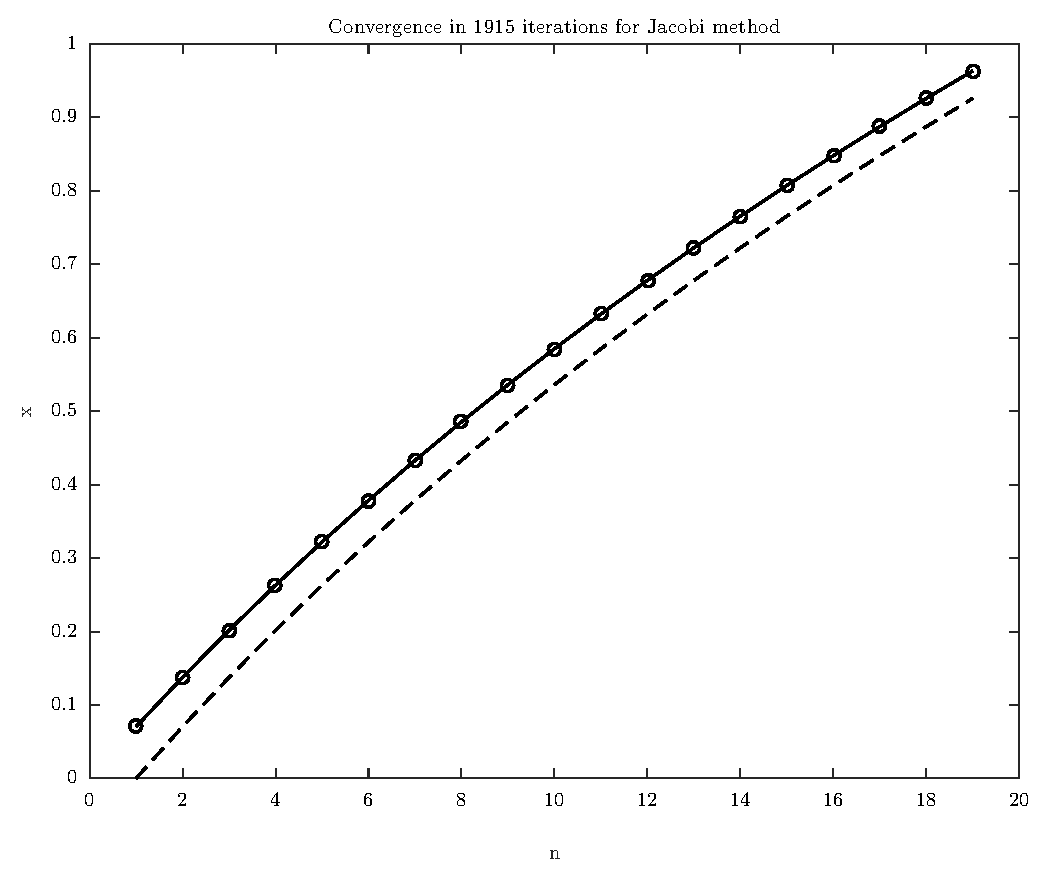
\includegraphics[width=\linewidth]{math609_pa2_comp_example_1_n_19_k_Jacobi_part_a.eps}
%\caption{Caption for figure 1}
\label{fig:test1}
\end{minipage}\hfill
\begin{minipage}{.45\textwidth}
\centering
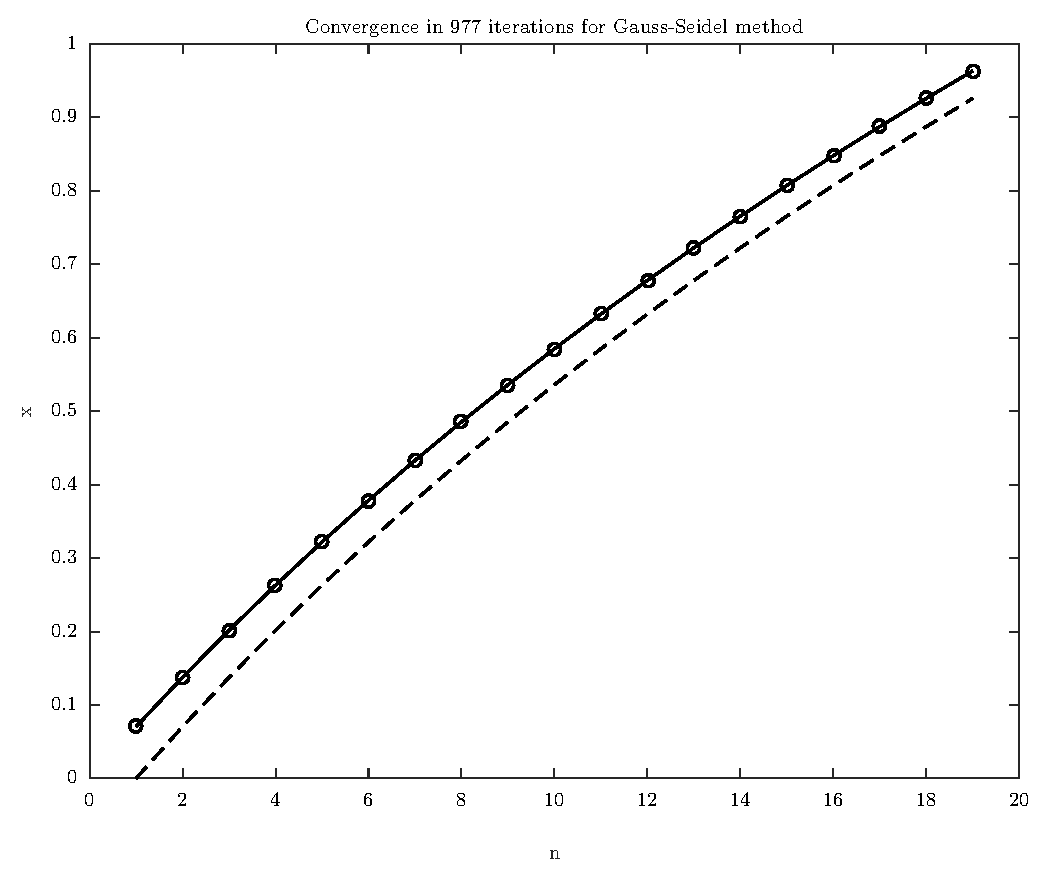
\includegraphics[width=\linewidth]{math609_pa2_comp_example_1_n_19_k_Gauss-Seidel_part_a.eps}
%\caption{Caption for figure 2}
\label{fig:test2}
\end{minipage}\hfill
\\
\begin{minipage}{.45\textwidth}
\centering
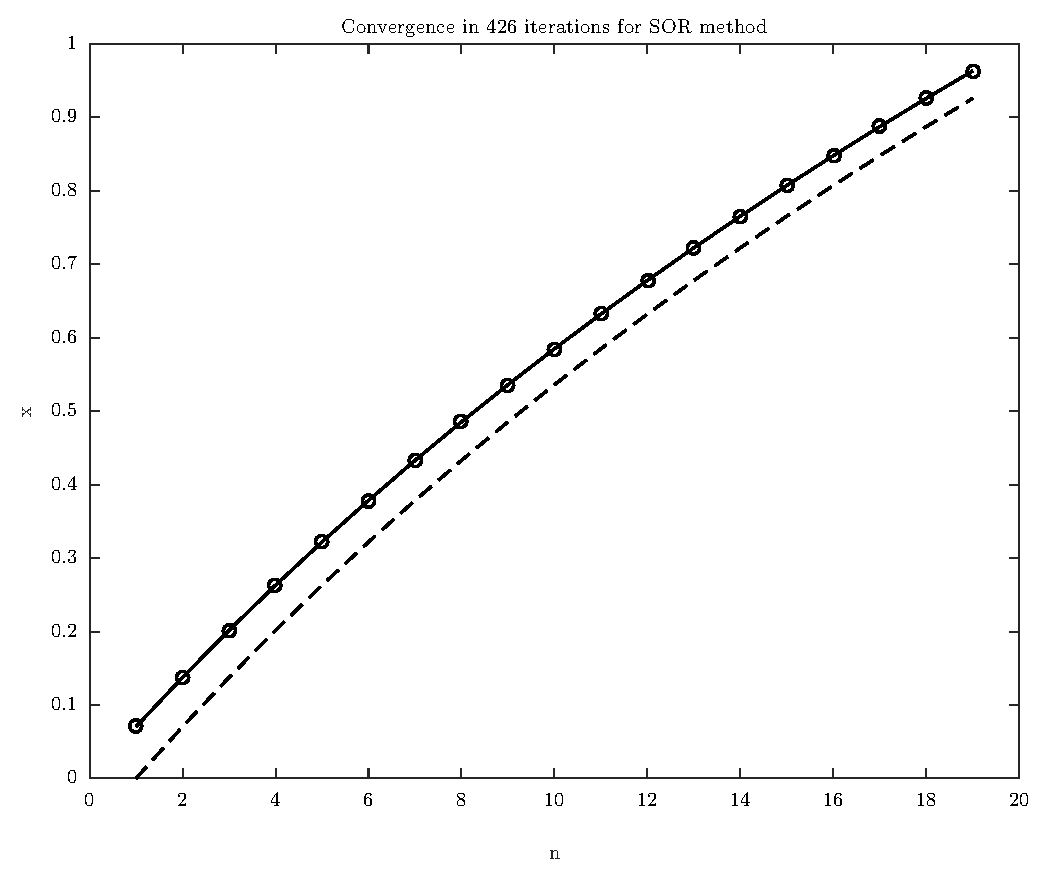
\includegraphics[width=\linewidth]{math609_pa2_comp_example_1_n_19_k_SOR_part_a.eps}
%\caption{Caption for figure 3}
\label{fig:test3}
\end{minipage}\hfill
\begin{minipage}{.45\textwidth}
\centering
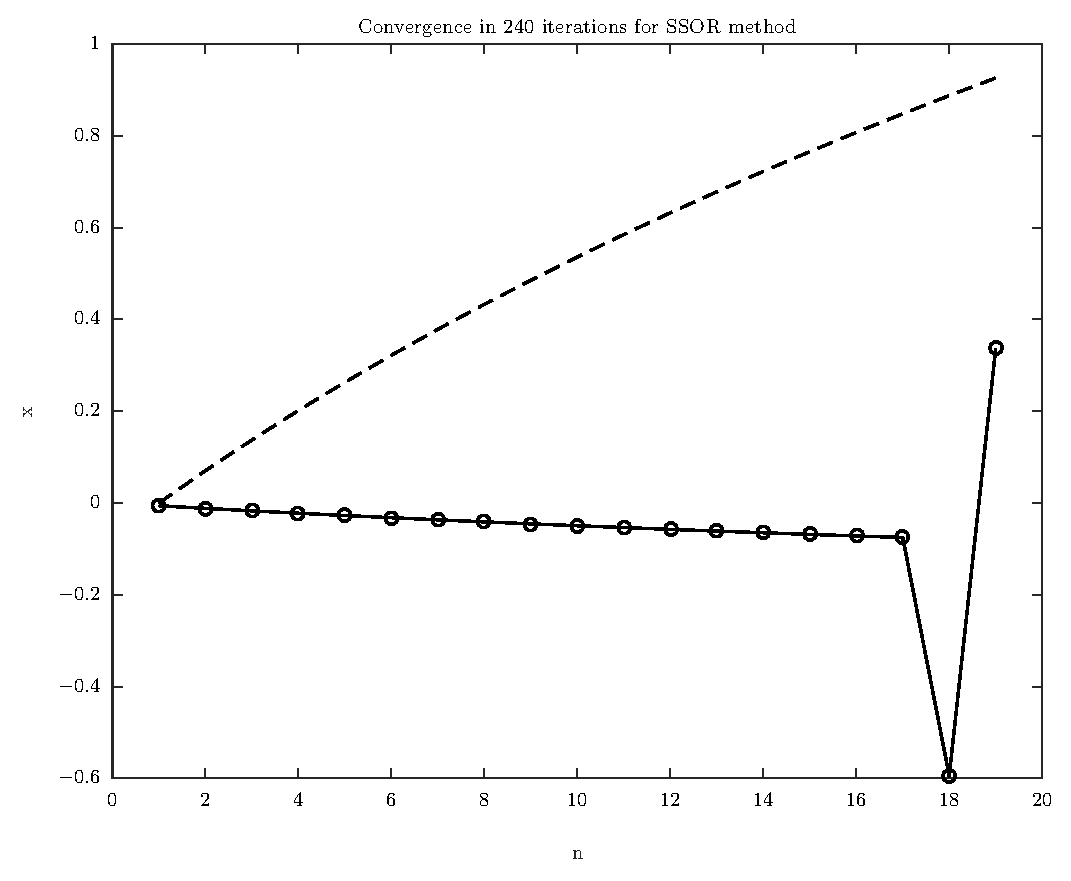
\includegraphics[width=\linewidth]{math609_pa2_comp_example_1_n_19_k_SSOR_part_a.eps}
%\caption{Caption for figure 3}
\label{fig:test3}
\end{minipage}\hfill
\caption{Comparative plots at n = 19}
\end{figure}
%%%%%%%%%%%%%%
\begin{figure}
\centering
\begin{minipage}{.45\textwidth}
\centering
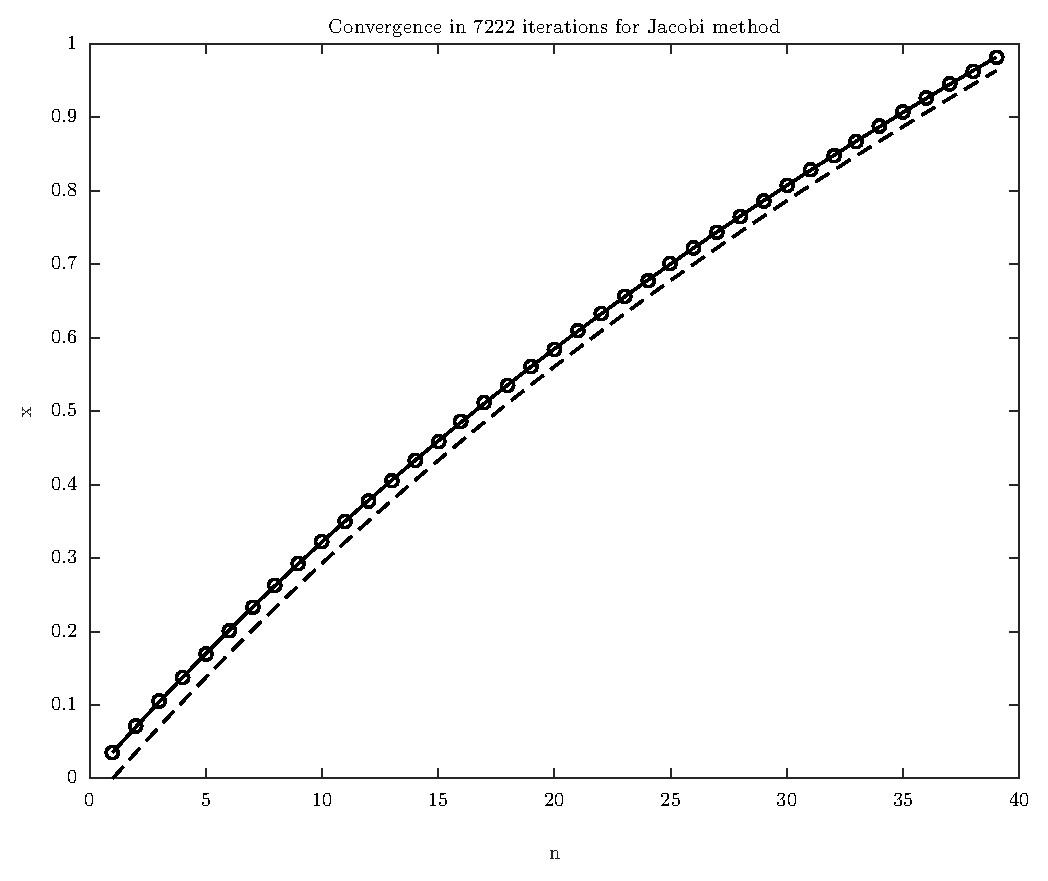
\includegraphics[width=\linewidth]{math609_pa2_comp_example_1_n_39_k_Jacobi_part_a.eps}
%\caption{Caption for figure 1}
\label{fig:test1}
\end{minipage}\hfill
\begin{minipage}{.45\textwidth}
\centering
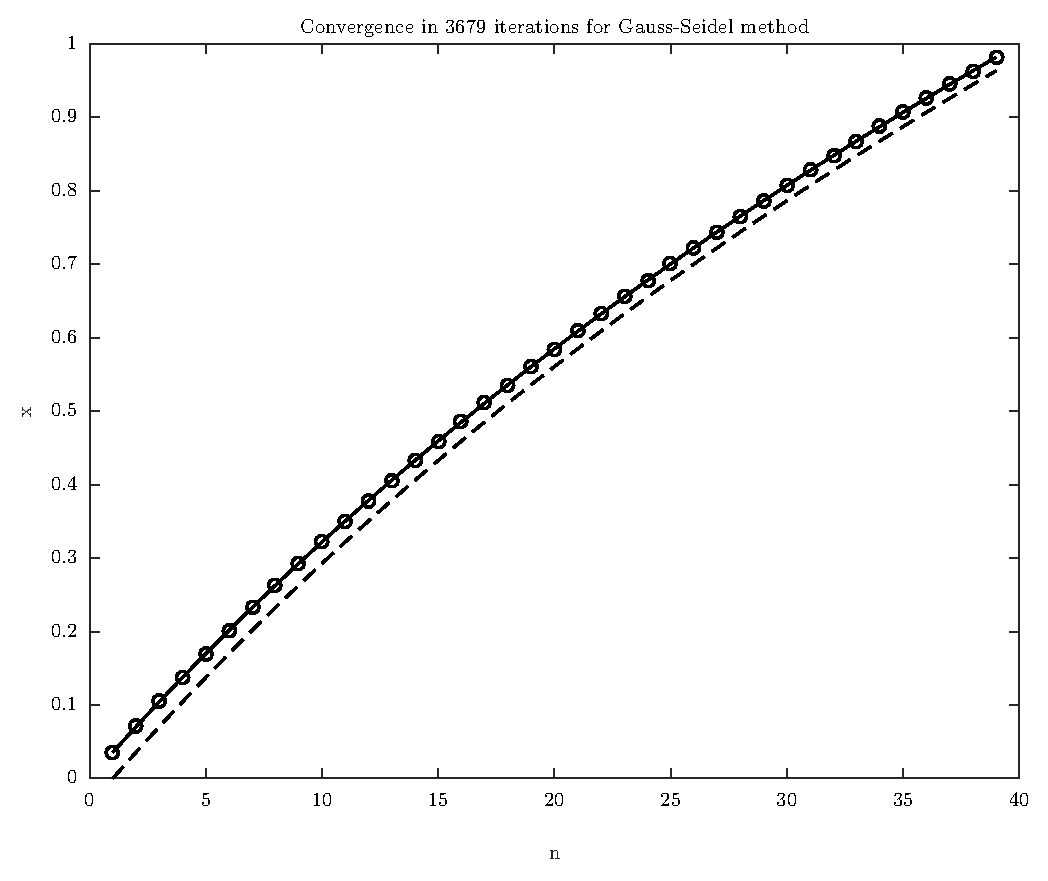
\includegraphics[width=\linewidth]{math609_pa2_comp_example_1_n_39_k_Gauss-Seidel_part_a.eps}
%\caption{Caption for figure 2}
\label{fig:test2}
\end{minipage}\hfill
\\
\begin{minipage}{.45\textwidth}
\centering
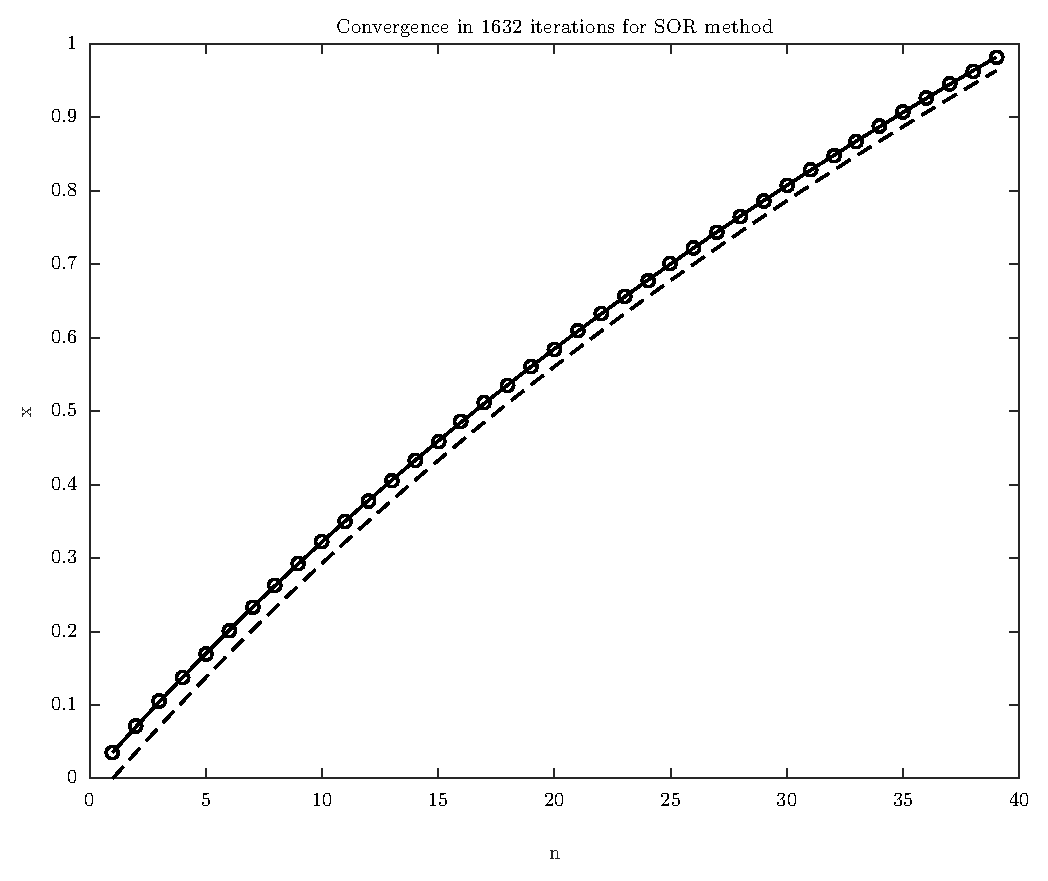
\includegraphics[width=\linewidth]{math609_pa2_comp_example_1_n_39_k_SOR_part_a.eps}
%\caption{Caption for figure 3}
\label{fig:test3}
\end{minipage}\hfill
\begin{minipage}{.45\textwidth}
\centering
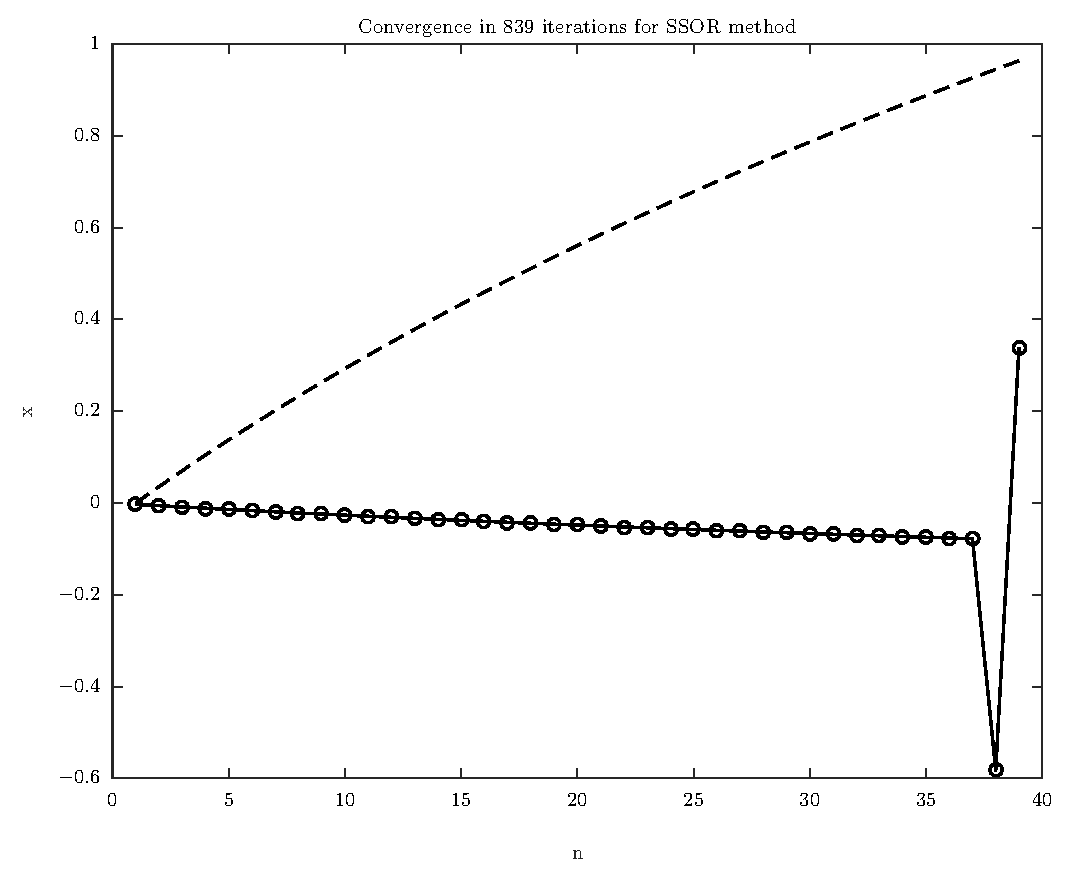
\includegraphics[width=\linewidth]{math609_pa2_comp_example_1_n_39_k_SSOR_part_a.eps}
%\caption{Caption for figure 3}
\label{fig:test3}
\end{minipage}\hfill
\caption{Comparative plots at n = 39}
\end{figure}
%%%%%%%%%%%%%%%%%%%%
\begin{figure}
\centering
\begin{minipage}{.45\textwidth}
\centering
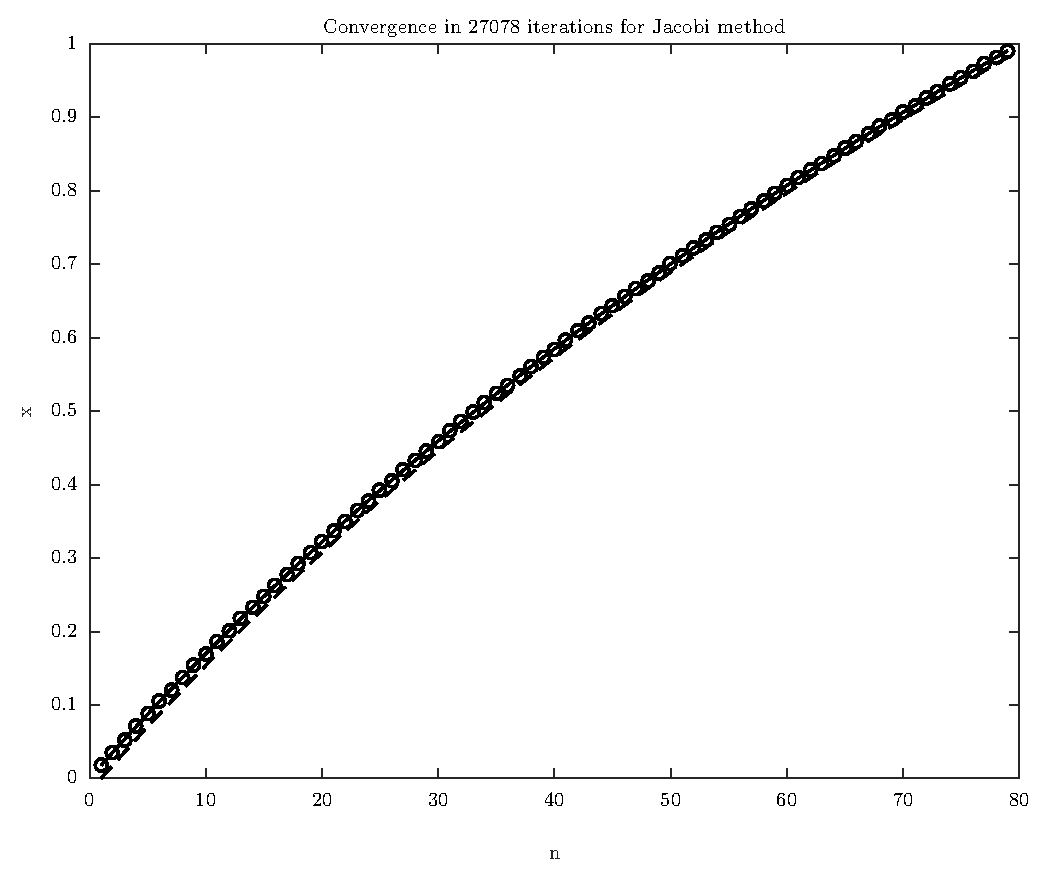
\includegraphics[width=\linewidth]{math609_pa2_comp_example_1_n_79_k_Jacobi_part_a.eps}
%\caption{Caption for figure 1}
\label{fig:test1}
\end{minipage}\hfill
\begin{minipage}{.45\textwidth}
\centering
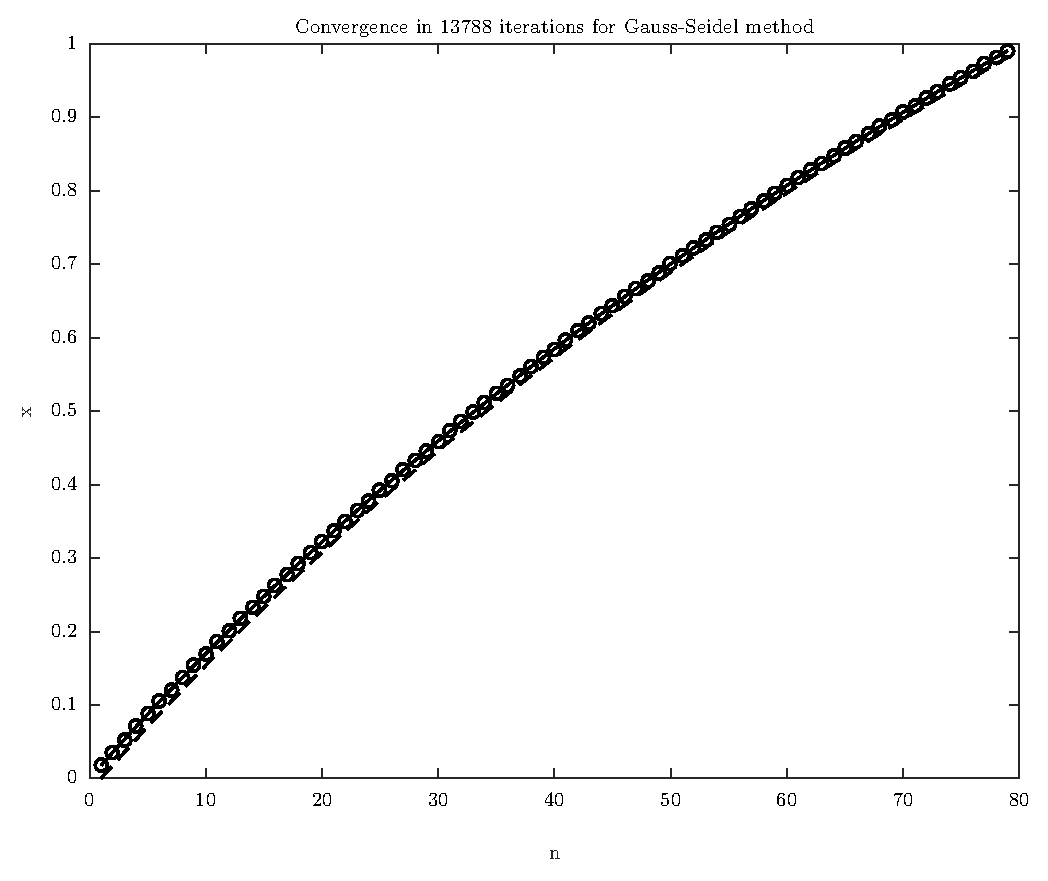
\includegraphics[width=\linewidth]{math609_pa2_comp_example_1_n_79_k_Gauss-Seidel_part_a.eps}
%\caption{Caption for figure 2}
\label{fig:test2}
\end{minipage}\hfill
\\
\begin{minipage}{.45\textwidth}
\centering
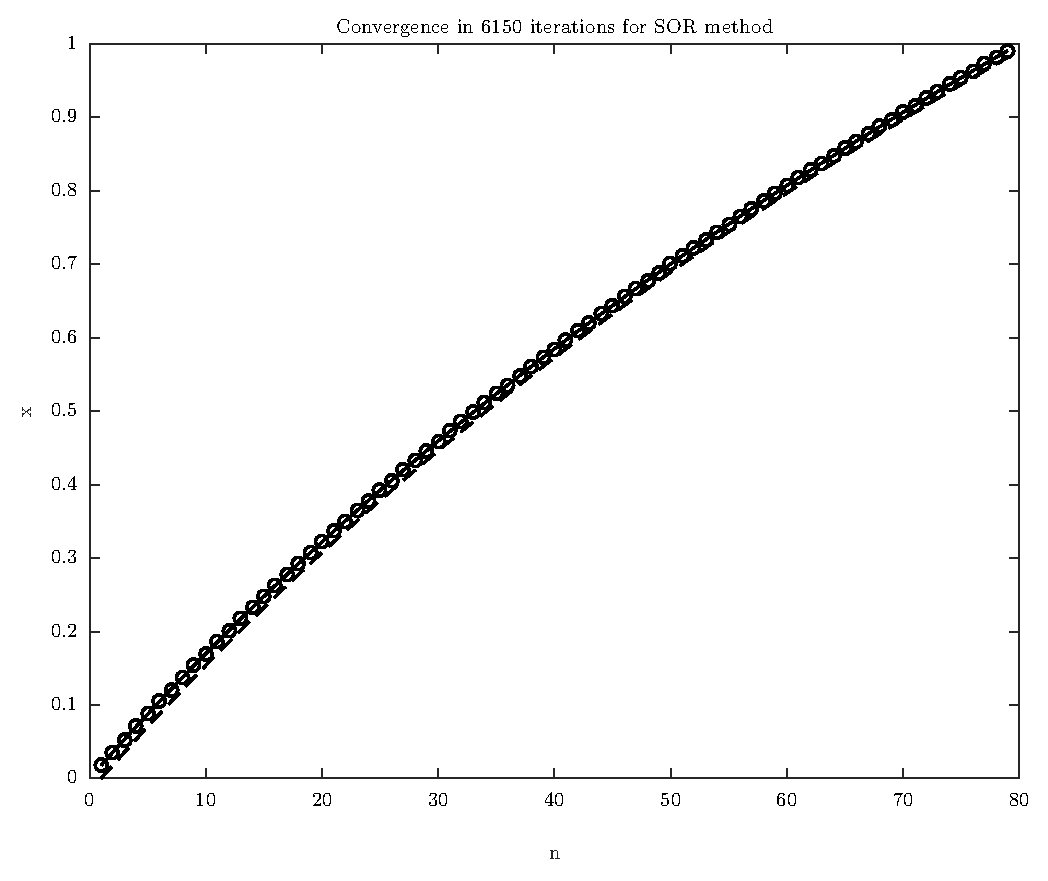
\includegraphics[width=\linewidth]{math609_pa2_comp_example_1_n_79_k_SOR_part_a.eps}
%\caption{Caption for figure 3}
\label{fig:test3}
\end{minipage}\hfill
\begin{minipage}{.45\textwidth}
\centering
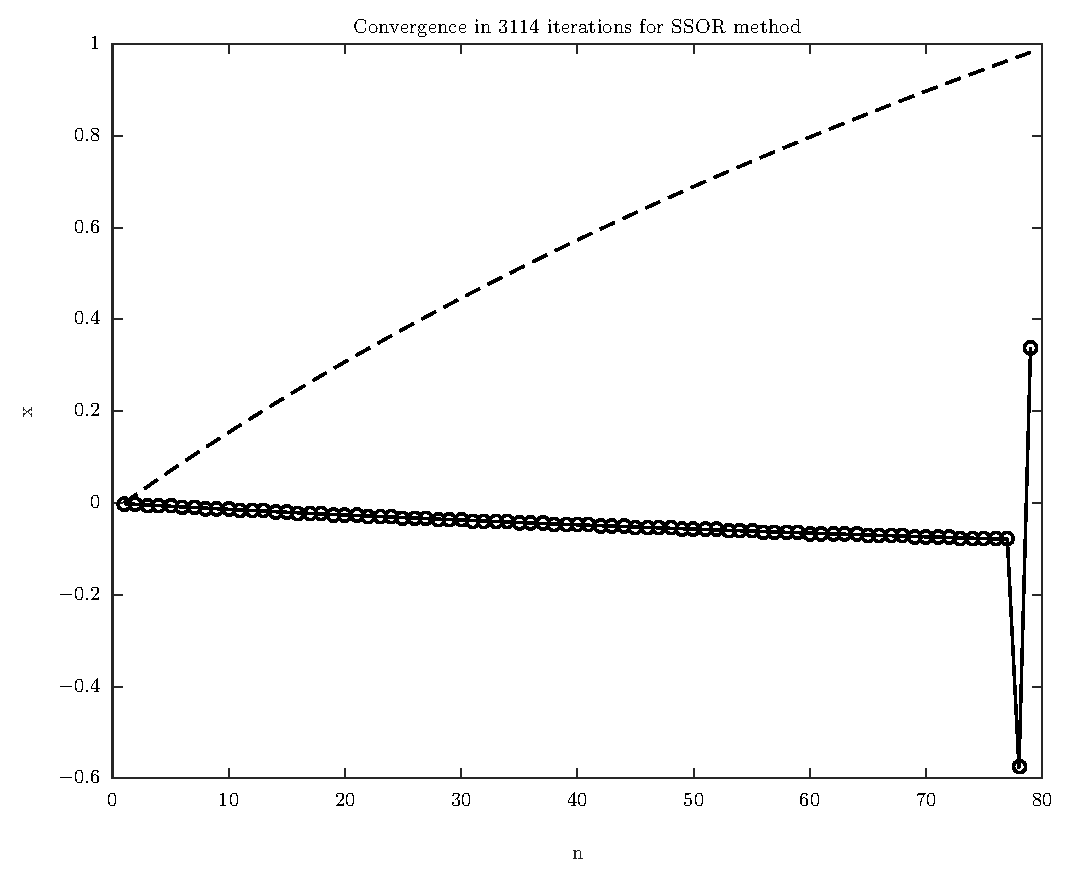
\includegraphics[width=\linewidth]{math609_pa2_comp_example_1_n_79_k_SSOR_part_a.eps}
%\caption{Caption for figure 3}
\label{fig:test3}
\end{minipage}\hfill
\caption{Comparative plots at n = 79}
\end{figure}
%%%%%%%%%%%%%%%%%%%%
%%%%%%%%%%%%%%%%%%%%
\begin{figure}
\centering
\begin{minipage}{.45\textwidth}
\centering
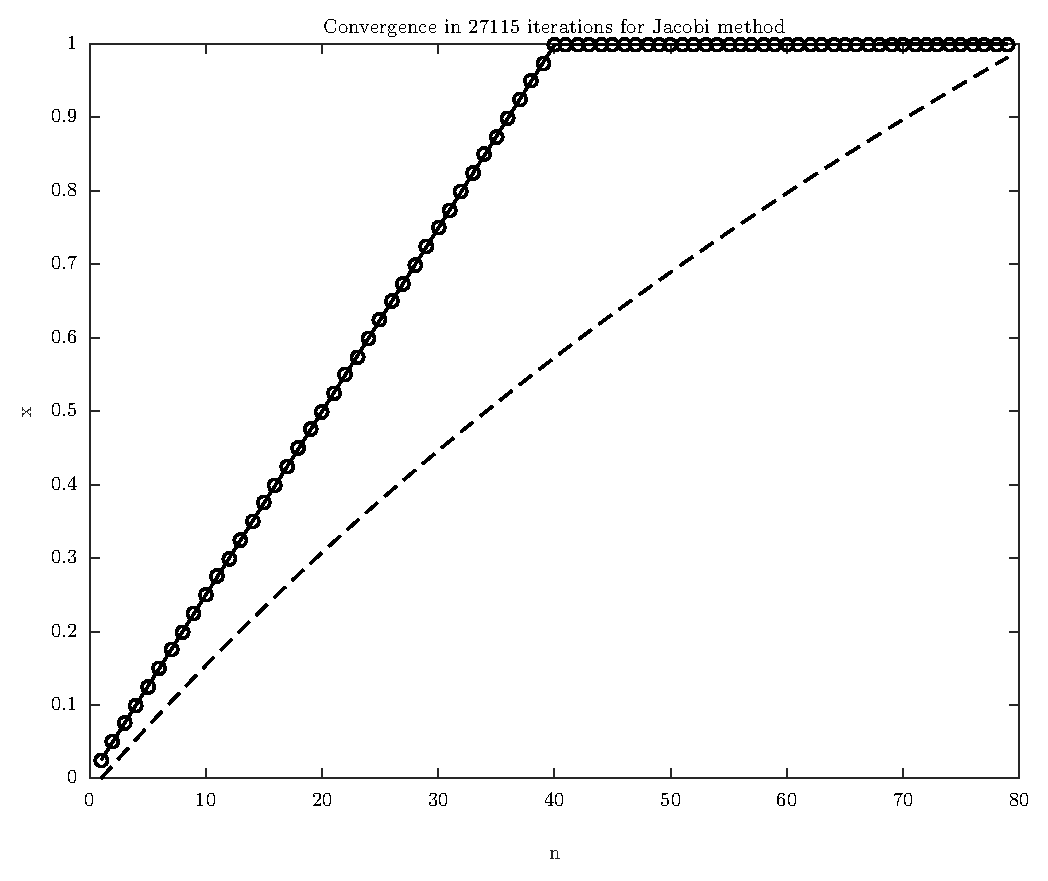
\includegraphics[width=\linewidth]{math609_pa2_comp_example_1_n_79_k_Jacobi_part_b.eps}
%\caption{Caption for figure 1}
\label{fig:test1}
\end{minipage}\hfill
\begin{minipage}{.45\textwidth}
\centering
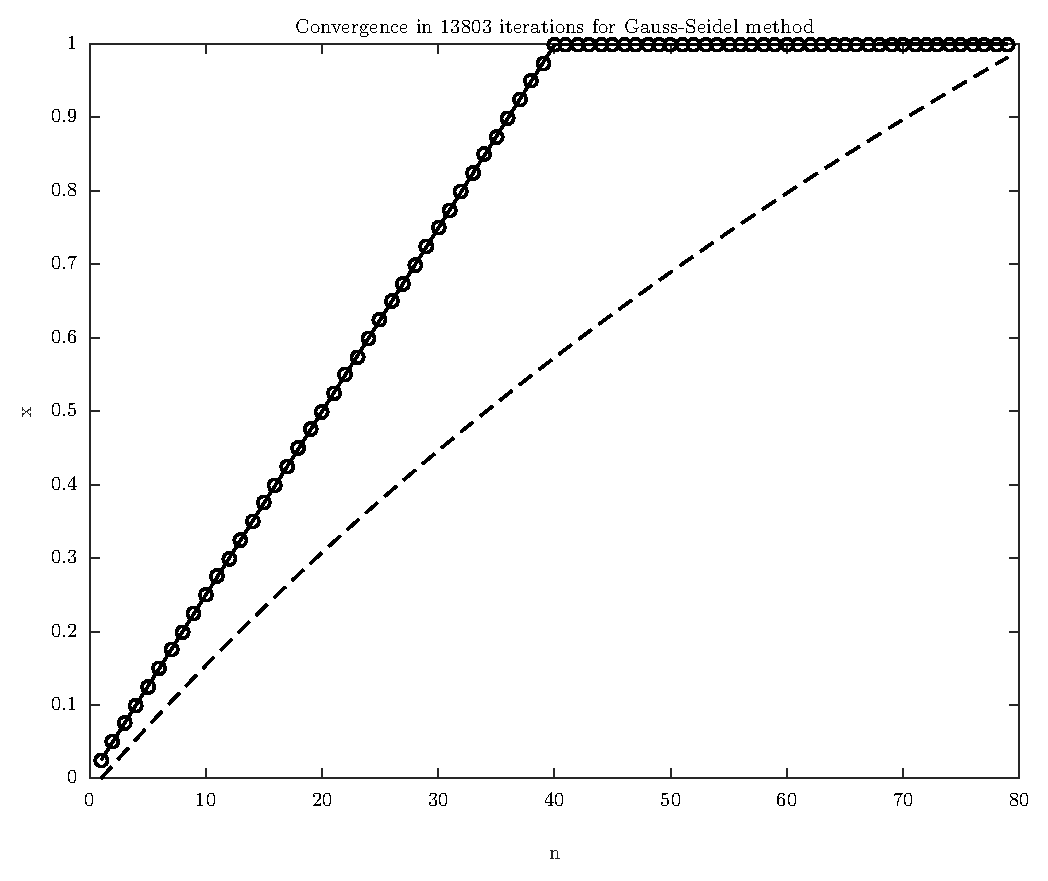
\includegraphics[width=\linewidth]{math609_pa2_comp_example_1_n_79_k_Gauss-Seidel_part_b.eps}
%\caption{Caption for figure 2}
\label{fig:test2}
\end{minipage}\hfill
\\
\begin{minipage}{.45\textwidth}
\centering
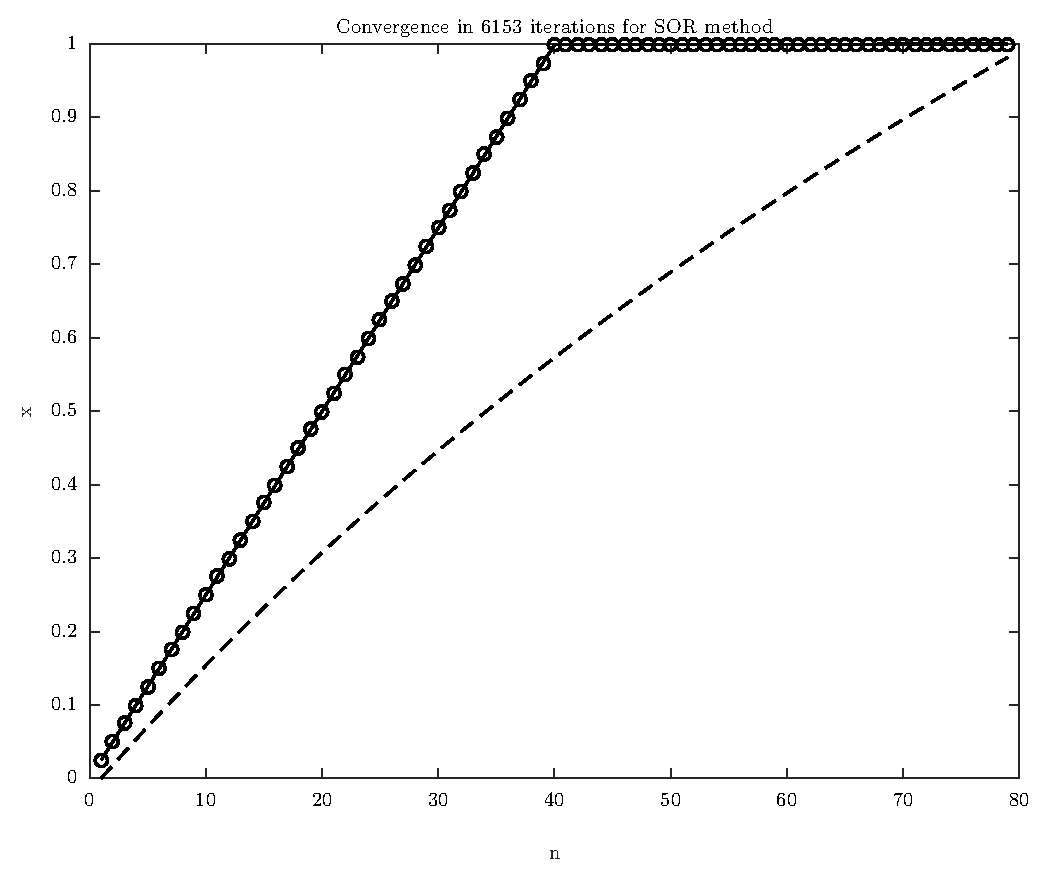
\includegraphics[width=\linewidth]{math609_pa2_comp_example_1_n_79_k_SOR_part_b.eps}
%\caption{Caption for figure 3}
\label{fig:test3}
\end{minipage}\hfill
\begin{minipage}{.45\textwidth}
\centering
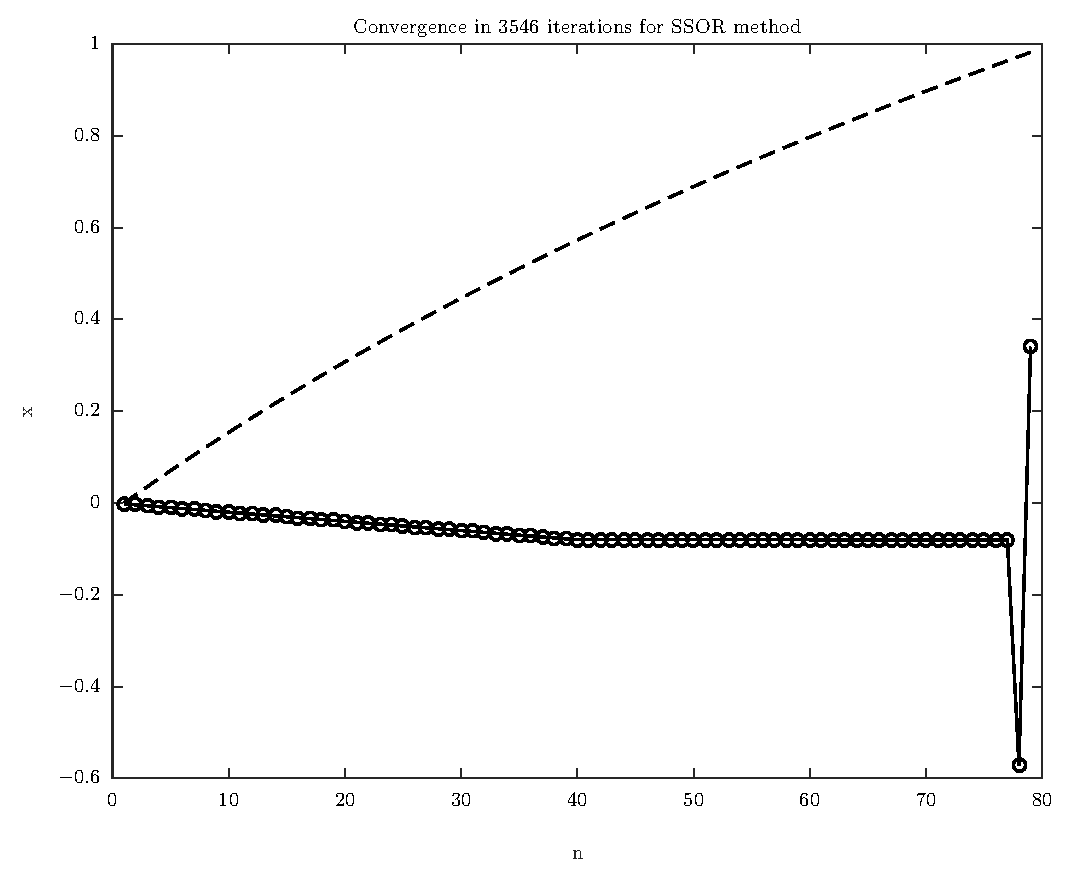
\includegraphics[width=\linewidth]{math609_pa2_comp_example_1_n_79_k_SSOR_part_b.eps}
%\caption{Caption for figure 3}
\label{fig:test3}
\end{minipage}\hfill
\caption{Comparative plots at n = 79}
\end{figure}
%%%%%%%%%%%%%%%%%%%%
%%%%%%%%%%%
%%%%%%%%%%%%%
%%%%%%%%%%%%
%%%%%%%%%%%%%%%%%%%%
\begin{figure}
\centering
\begin{minipage}{.45\textwidth}
\centering
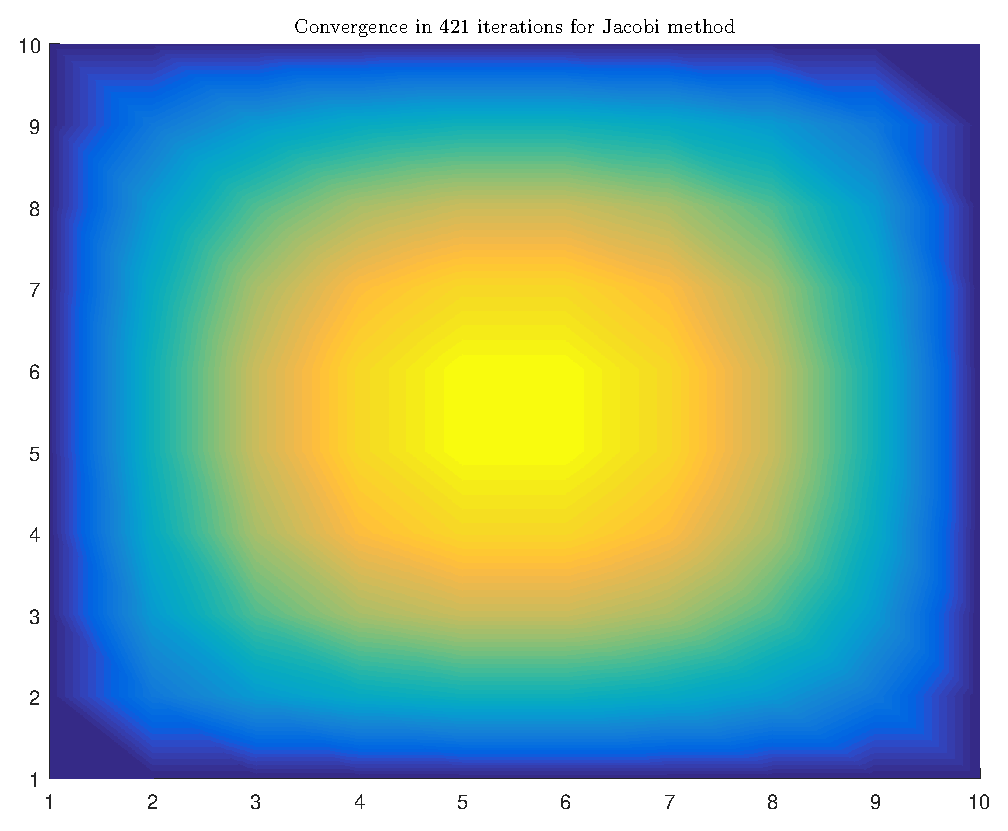
\includegraphics[width=\linewidth]{math609_pa2_comp_example_2_8_n_Jacobi.eps}
%\caption{Caption for figure 1}
\label{fig:test1}
\end{minipage}\hfill
\begin{minipage}{.45\textwidth}
\centering
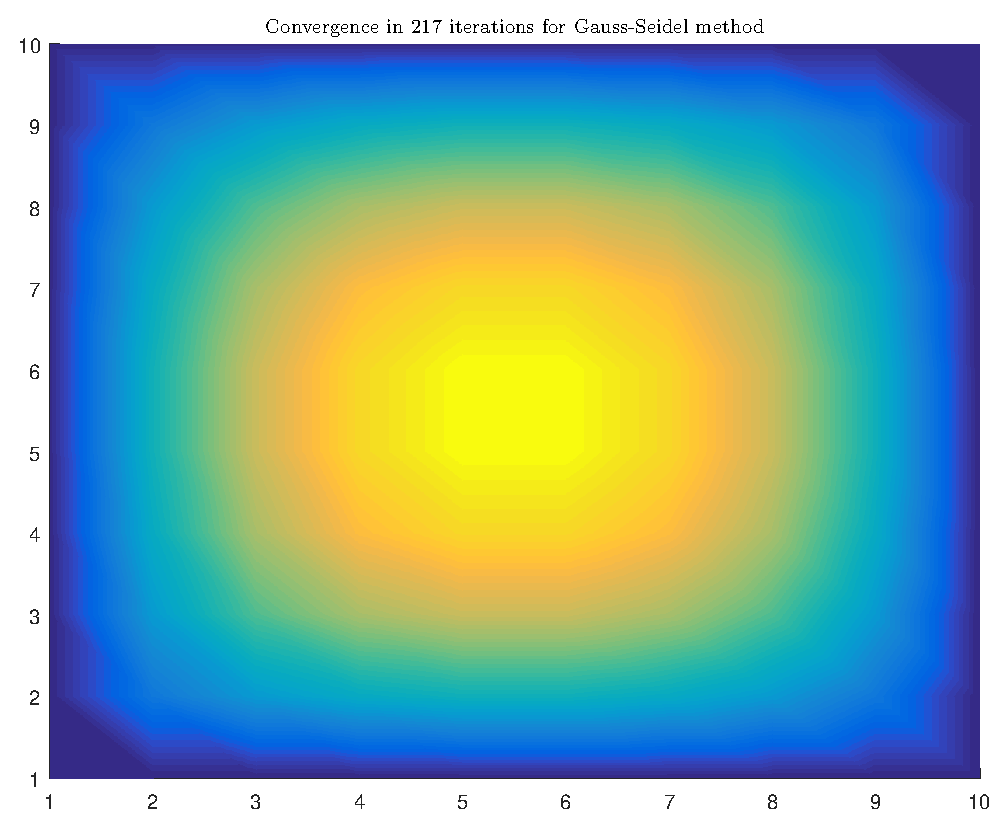
\includegraphics[width=\linewidth]{math609_pa2_comp_example_2_8_n_Gauss-Seidel.eps}
%\caption{Caption for figure 2}
\label{fig:test2}
\end{minipage}\hfill
\\
\begin{minipage}{.45\textwidth}
\centering
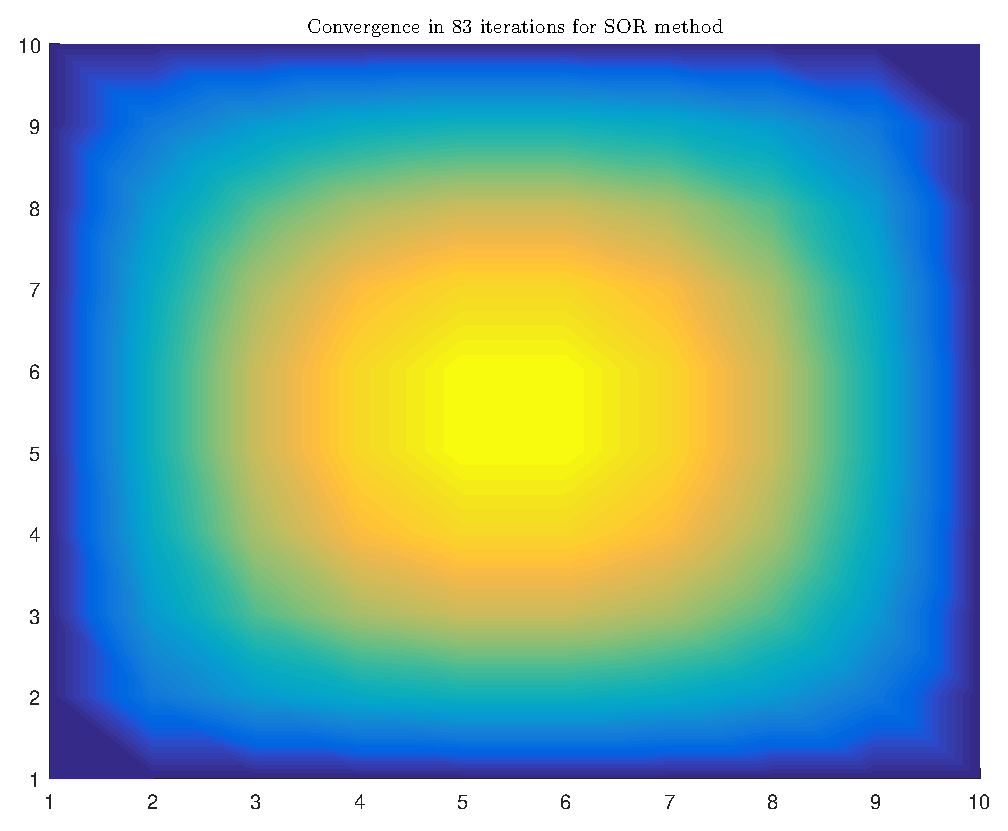
\includegraphics[width=\linewidth]{math609_pa2_comp_example_2_8_n_SOR.eps}
%\caption{Caption for figure 3}
\label{fig:test3}
\end{minipage}\hfill
\begin{minipage}{.45\textwidth}
\centering
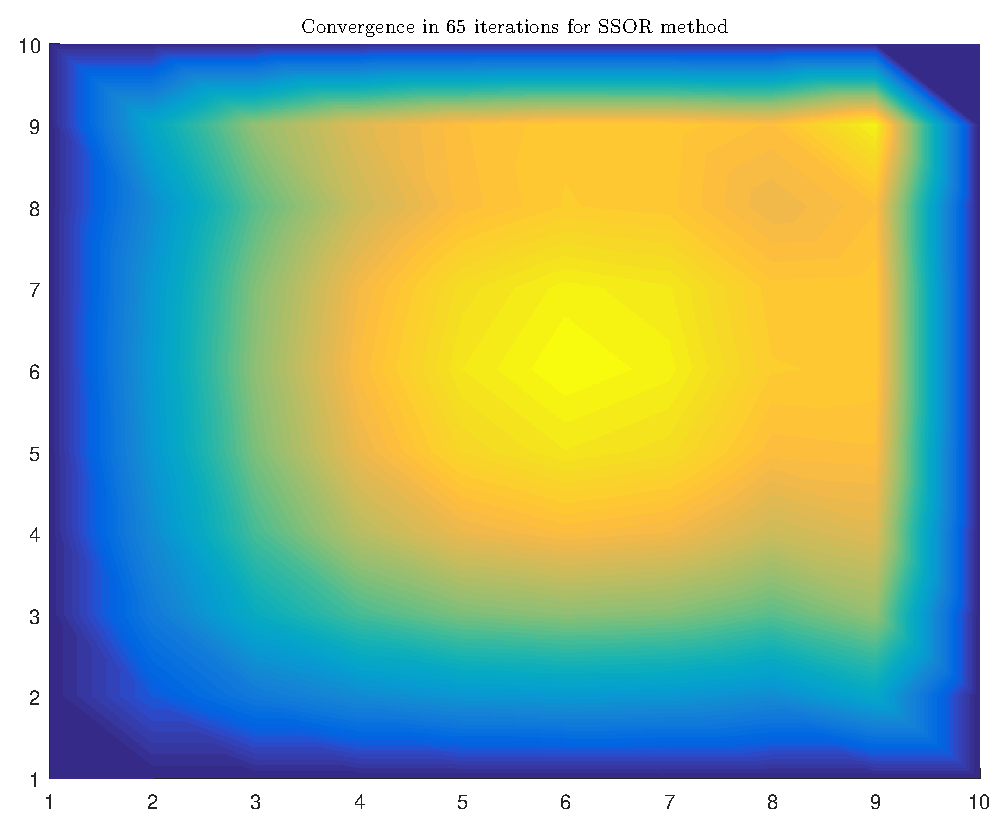
\includegraphics[width=\linewidth]{math609_pa2_comp_example_2_8_n_SSOR.eps}
%\caption{Caption for figure 3}
\label{fig:test3}
\end{minipage}\hfill
\caption{Surface Plots of Five-point Finite Difference Equation solution at n = 8}
\end{figure}
%%%%%%%%%%%%%%%%%%%%
%%%%%%%%%%%%%%%%%%%%

\begin{figure}
\centering
\begin{minipage}{.45\textwidth}
\centering
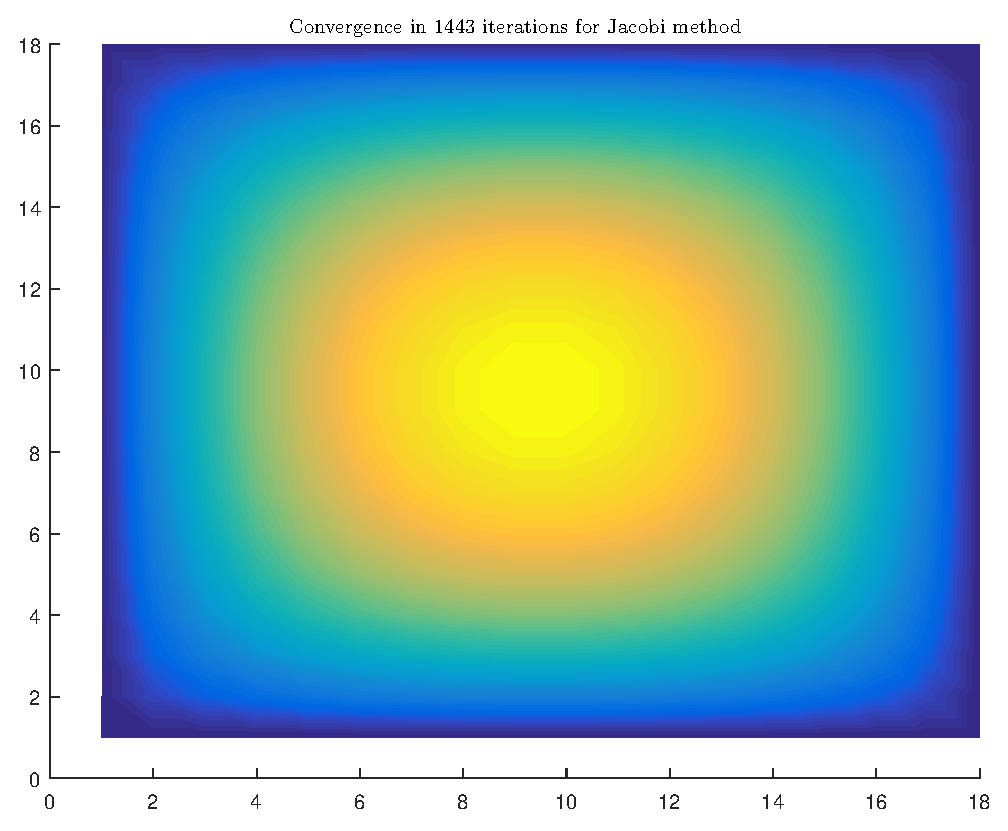
\includegraphics[width=\linewidth]{math609_pa2_comp_example_2_16_n_Jacobi.eps}
%\caption{Caption for figure 1}
\label{fig:test1}
\end{minipage}\hfill
\begin{minipage}{.45\textwidth}
\centering
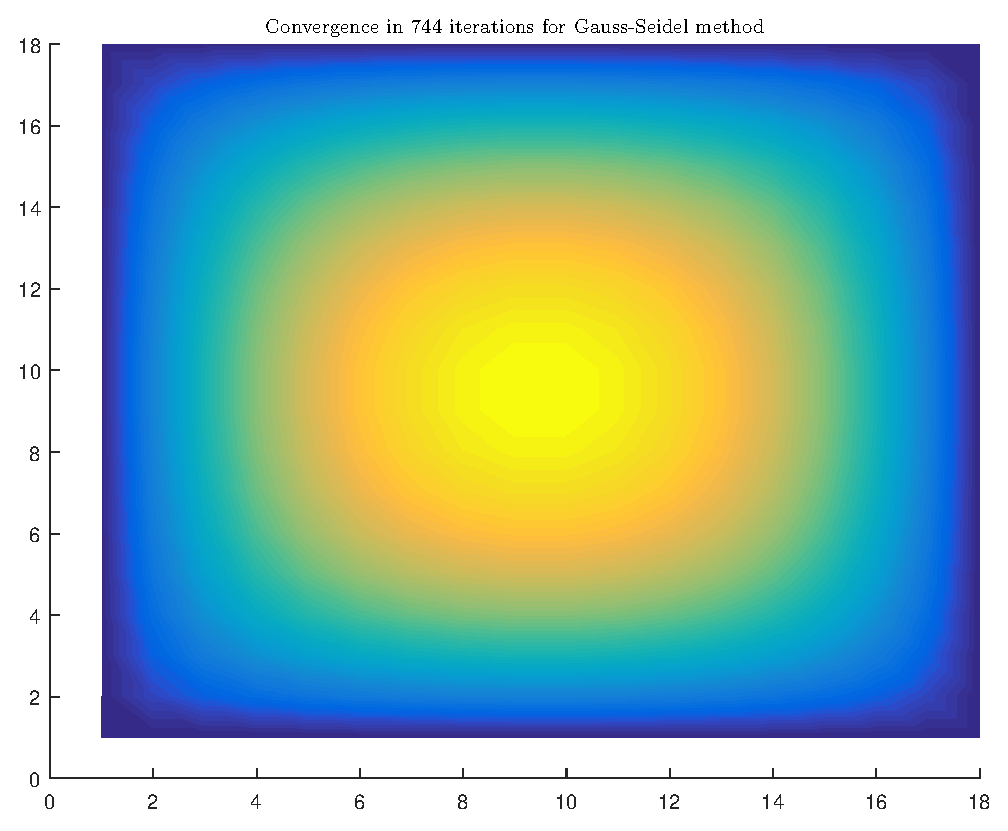
\includegraphics[width=\linewidth]{math609_pa2_comp_example_2_16_n_Gauss-Seidel.eps}
%\caption{Caption for figure 2}
\label{fig:test2}
\end{minipage}\hfill
\\
\begin{minipage}{.45\textwidth}
\centering
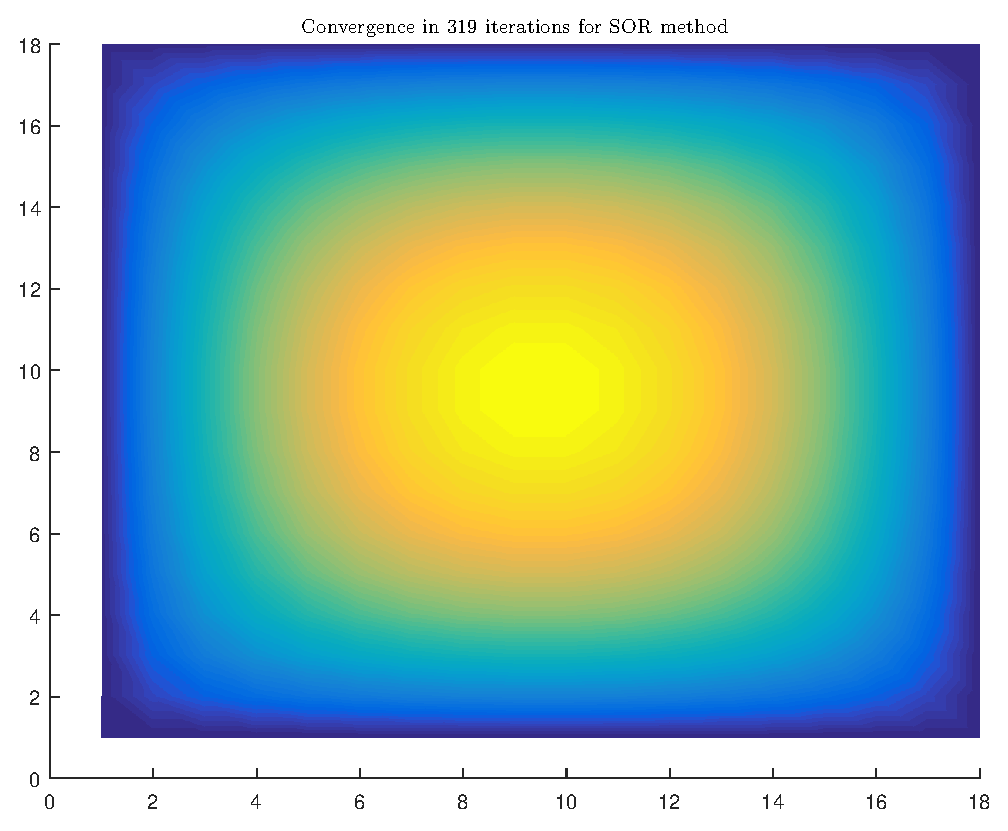
\includegraphics[width=\linewidth]{math609_pa2_comp_example_2_16_n_SOR.eps}
%\caption{Caption for figure 3}
\label{fig:test3}
\end{minipage}\hfill
\begin{minipage}{.45\textwidth}
\centering
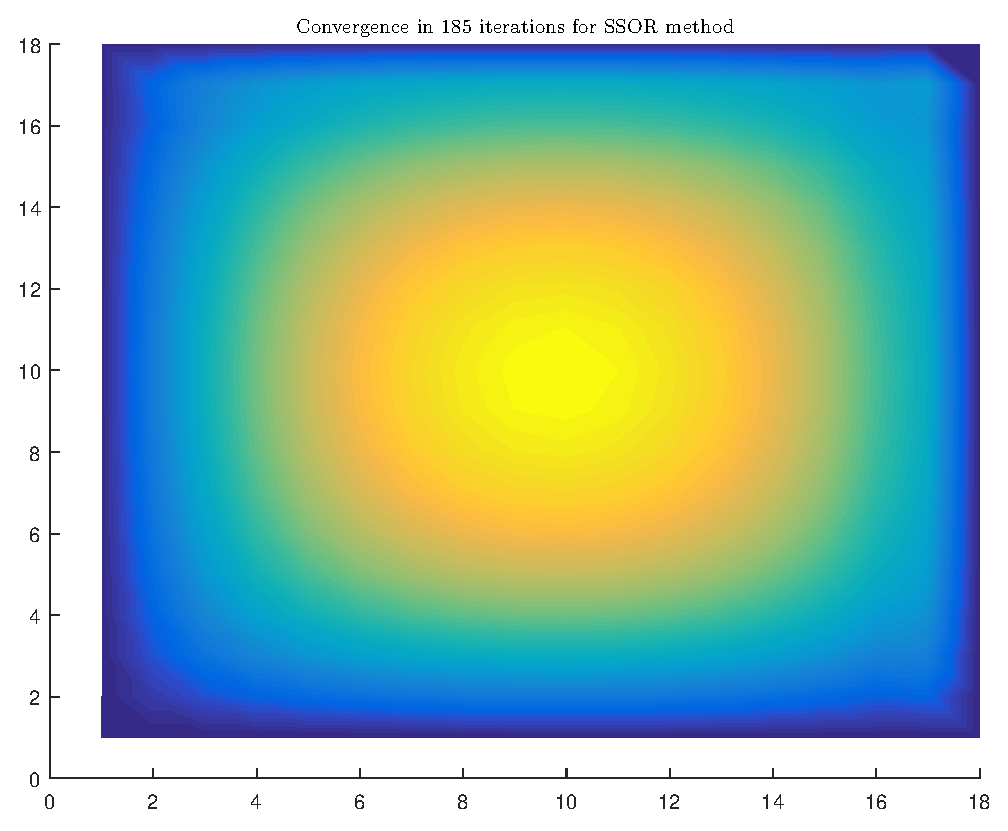
\includegraphics[width=\linewidth]{math609_pa2_comp_example_2_16_n_SSOR.eps}
%\caption{Caption for figure 3}
\label{fig:test3}
\end{minipage}\hfill
\caption{Surface Plots of Five-point Finite Difference Equation solution at n = 16}
\end{figure}
%%%%%%%%%%%%%%%%%%%%
\begin{figure}
\centering
\begin{minipage}{.45\textwidth}
\centering
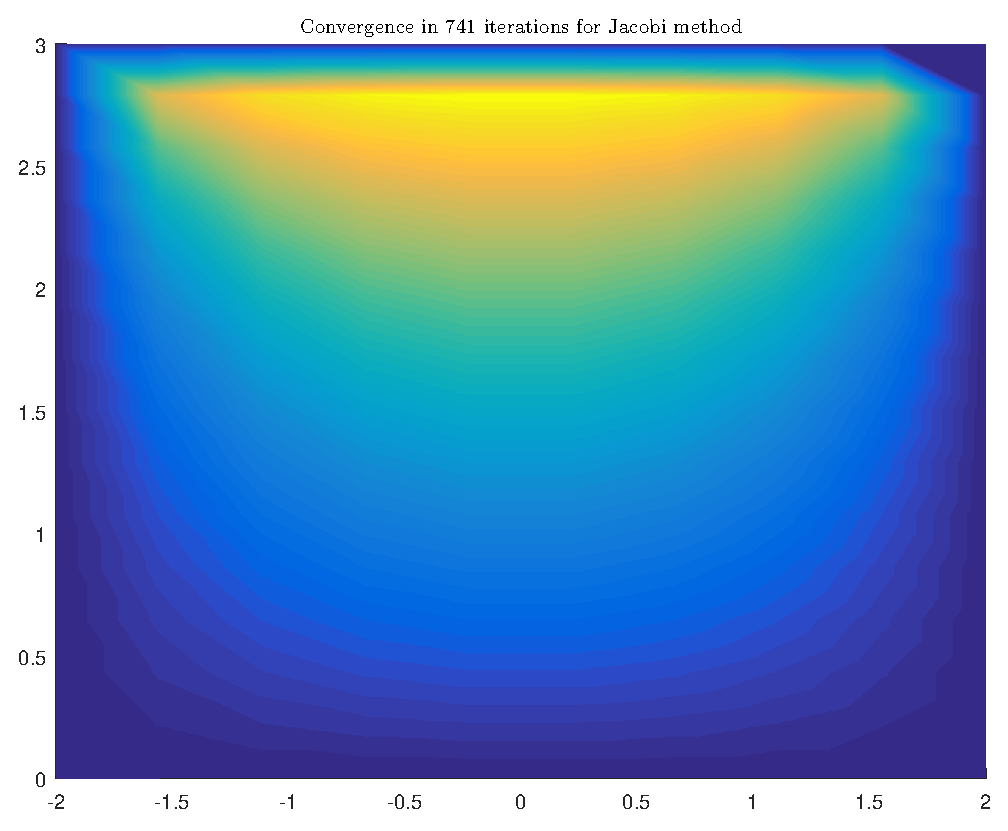
\includegraphics[width=\linewidth]{math609_pa3_comp_example_2_104_n_Jacobi.eps}
%\caption{Caption for figure 1}
\label{fig:test1}
\end{minipage}\hfill
\begin{minipage}{.45\textwidth}
\centering
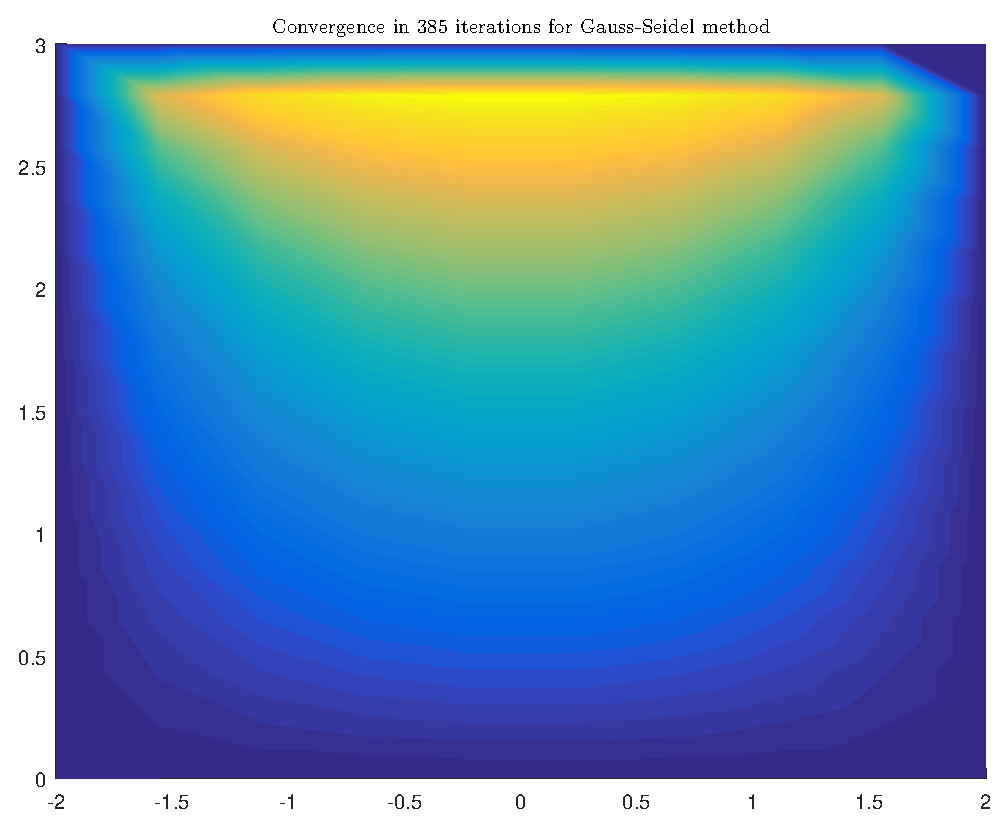
\includegraphics[width=\linewidth]{math609_pa3_comp_example_2_104_n_Gauss-Seidel.eps}
%\caption{Caption for figure 2}
\label{fig:test2}
\end{minipage}\hfill
\\
\begin{minipage}{.45\textwidth}
\centering
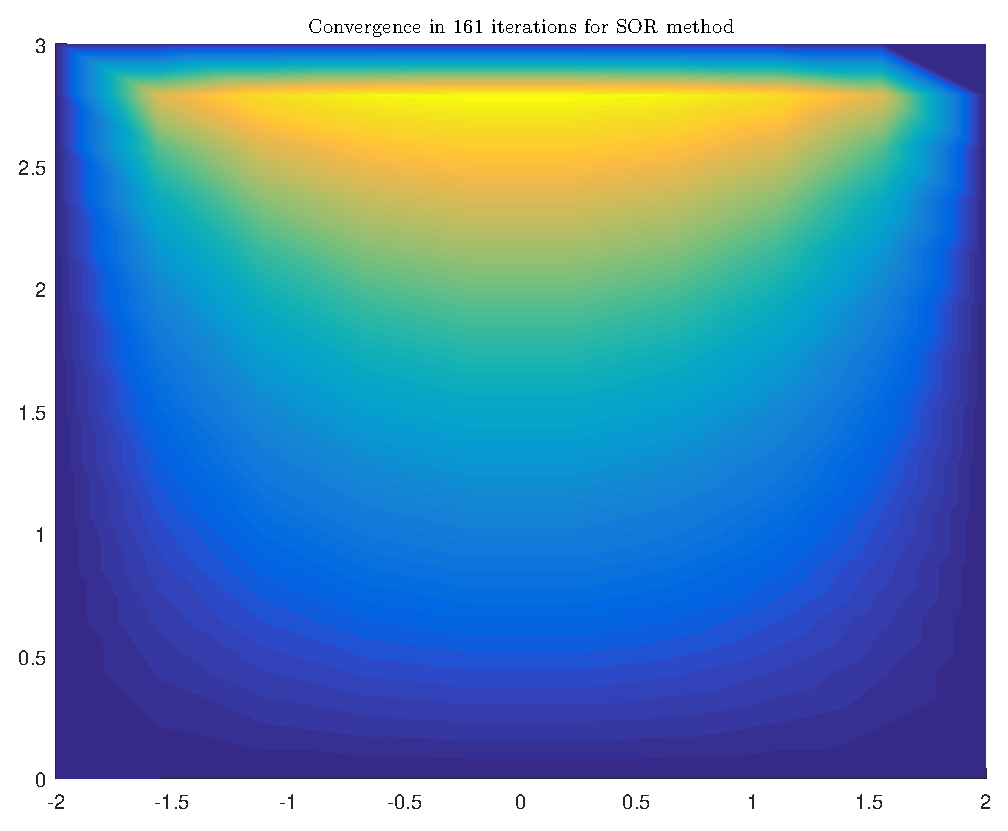
\includegraphics[width=\linewidth]{math609_pa3_comp_example_2_104_n_SOR.eps}
%\caption{Caption for figure 3}
\label{fig:test3}
\end{minipage}\hfill
\begin{minipage}{.45\textwidth}
\centering
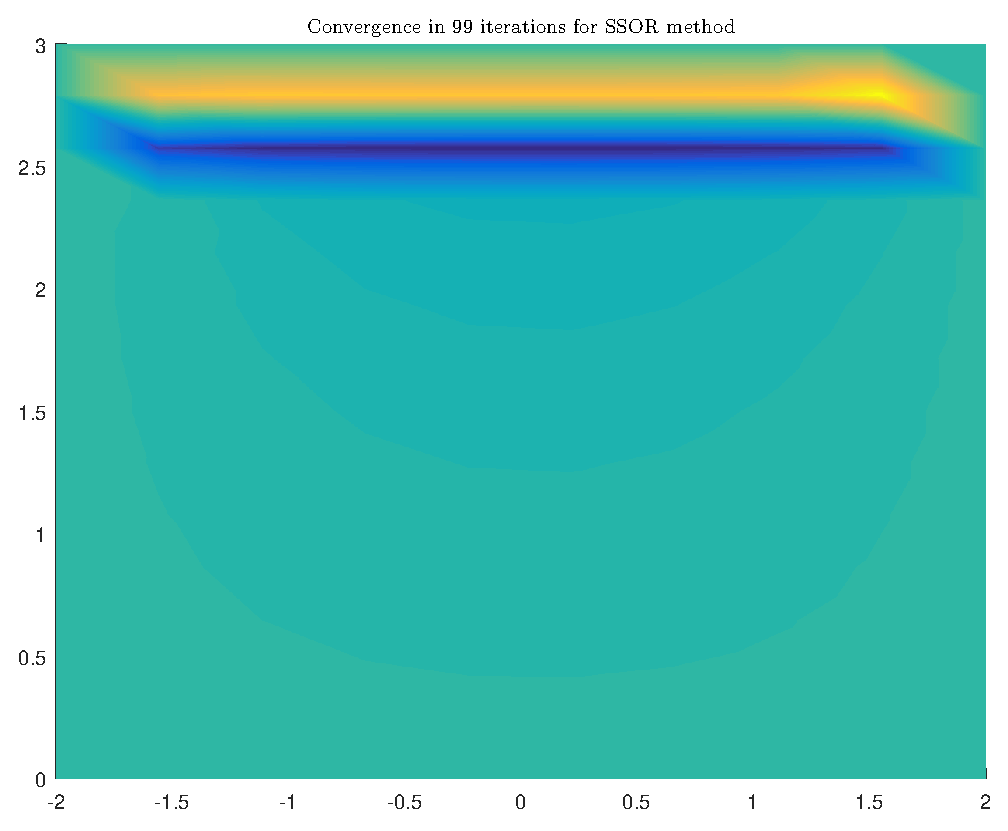
\includegraphics[width=\linewidth]{math609_pa3_comp_example_2_104_n_SSOR.eps}
%\caption{Caption for figure 3}
\label{fig:test3}
\end{minipage}\hfill
\caption{Surface Plots of Five-point Finite Difference Equation solution at nx = 10 and ny = 15}
\end{figure}
%%%%%%%%%%%%%%%%%%%%
%%%%%%%%%%%%%%%%%%%%




\end{document}








